\documentclass[../mattg_ti-fi_lit-review.tex]{subfiles}

\subsection{Synthesis, Growth and Fabrication}
\textcolor{red}{TODO: fill in with summary of previous growth methods and experimental methods used for heterostructures}.
\subsubsection{MBE Growths}

\subsection{Spectroscopic Metrological Methods}
\subsubsection{ARPES}\label{sec:ARPES}
For material characterisation, angle resolved photo-emission spectroscopy (ARPES) is a method of resolving the ejection of electrons from a material by high energy photons. Analysis of the momentum of the incident and emission resolve the electronic band structure.

There now exist a variety of different ARPES methods that can be employed in understanding the electronic structure of materials; these include ``soft-X-ray ARPES, time-resolved ARPES, spin-resolved ARPES and spatially resolved ARPES''\cite{lv_angle-resolved_2019}. The progress fo UV and soft-X-ray synchrotron light sources make it possible to distinguish between bulk and surface states for TI materials. Spin detectors determine the spin state of emitted electrons, allowing insight into spin-textures of surface states. Time-resolved ARPES (using femtosecond pulses) allows observation of ``ultrafast electronic dynamics and states above the chemical potential" \cite{lv_angle-resolved_2019}. Finally, spatially resolved ARPES can be used to pinpoint sub-micron scale features, particularly if you want to distinguish between phases, or across material gradients (such as gradient MBE growths).

\paragraph{Spin Resolved ARPES}\label{sec:ARPES-SR}
The first spin resolved (SR) ARPES that yielded the direct observation of helical spin-polarization was done by Hsieh \etal \cite{hsieh_observation_2009} at the end of 2008, again in \bismuthantimony{}, followed with more detailed results by Nishide \etal{}\cite{nishide_direct_2010}. 

In these experiments, topological details could be found by studying the surface band-dispersion and their respective spin polarizations. For example, the fact that there are 5 bands implies that an odd number of Fermi-surfaces enclose the spin-degenerate K points. This gives rise to determining the topological quantum number $\nu_0=1$ (0 if even). 

However Ando argued that these conclusions were questionable, due to purely relying on states already existing in Bismuth, which did not agree well with theoretical calculations \cite{ando_topological_2013}.

\subsubsection{Spin polarized STS}
The first scanning tunelling spectropscopy (STS) study on \bismuthantimony{} was published in 2009 by Roushan \etal{\cite{roushan_topological_2009}} who detected the absense of backscattering even with strong system disorder. By taking fourier transforms of the surface state data they take, they can infer scattering information and lattice information. Combining this with spin-resolved ARPES they could determine the spin dependent scattering probability, and match their STS measurements to 95\%. Doing the same with spin-independent scattering yields a match of only 80\%.

\subsection{Transport Metrological Methods}

\subsubsection{Quantum Oscillations}
Taskin \& Ando \cite{taskin_quantum_2009} used quantum behaviour reported in Bi and \bismuthantimony{} to differentiate between coherent electronic transport (edge states) and incoherent transport within an impurity band. The measurements (along with magnetic \& resistivity measurements) where implemented using the ``de Haas-van Alphen (dHvA)'' effect. To do this, you measure the magnetisation M across magnetic field strengths B. They also measured this quantity for different orientations of the sample, however it is also present in the bare resistivity of the sample.

\begin{figure}[H]
	\centering
	\begin{minipage}[t]{.95\textwidth}
		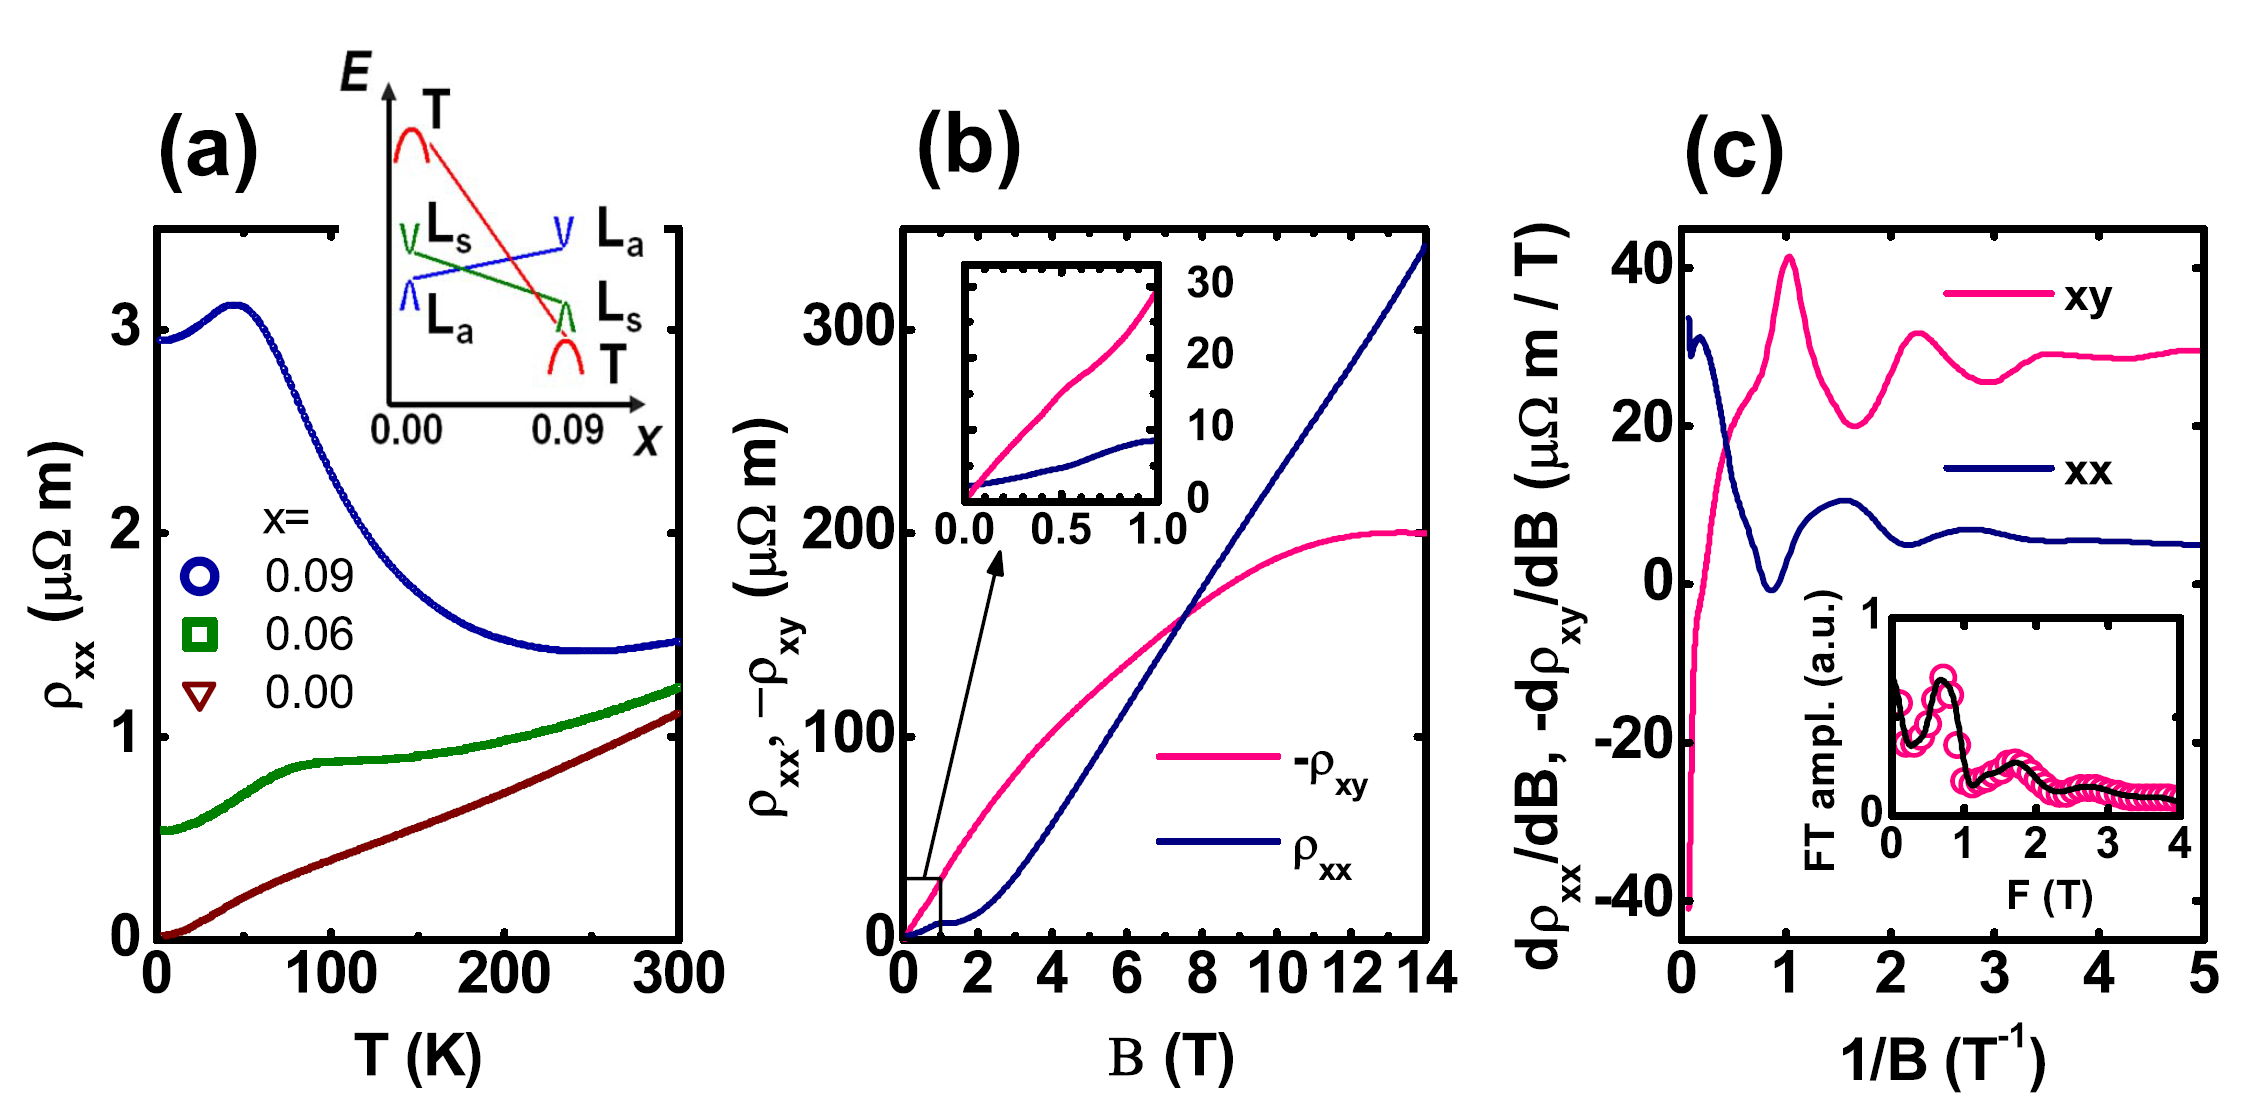
\includegraphics[width=\linewidth]{ti_bisb_qo}
		\caption{Observation of the quantum oscillations in \bismuthantimony{}.\\\textbf{a)} Temperature dependent $\rho_{xx}$ for different $x$. \textbf{b)} Magnetic field dependent $\rho_{xx}$ and $\rho_{xy}$ for x=0.09 @ 1.4K \textbf{c)} Derivatives of b), against $1/B$. Inset shows FT spectrum $-\rho_{xy}$.
			\\Source: Taskin and Ando\cite{taskin_quantum_2009} Phys. Rev. B 80, 085303 (2009)}
		\label{fig:ti_bisb_qo}
	\end{minipage}
\end{figure}


The derivative of the both $\rho_{xx}$ and $\rho_{xx}$ with respect to B, plotted against $1/B$ show Shubnikov-de Haas (SdH) oscillations below 2T field strength, as shown in Fig \ref{fig:ti_bisb_qo}c. This is a quantum effect, and consequently is argued that it comes from a well-defined Fermi surface, not some impurity band which wouldn't be stable. The previous measurements of the resistivity with different doping proportions confirmed the insulating nature of the samples.

\subsubsection{Magnetization}
Taskin \& Ando \cite{taskin_quantum_2009} measured DC magnetization using a SQUID magnetometer.